\documentclass[10pt,a4paper]{article}

% =========================
% Packages
% =========================
\usepackage[margin=1in]{geometry}
\usepackage[T1]{fontenc}
\usepackage[utf8]{inputenc}
\usepackage{newtxtext,newtxmath}   % Times-like font
\usepackage{microtype}
\usepackage{setspace}
\usepackage{graphicx}
\usepackage{booktabs}
\usepackage{multirow}
\usepackage{array}
\usepackage{amsmath,amssymb,amsthm}
\usepackage{algorithm}
\usepackage{algpseudocode}
\usepackage{caption}
\usepackage{subcaption}
\usepackage{enumitem}
\usepackage[numbers,sort&compress]{natbib}
\usepackage[hidelinks]{hyperref}
\usepackage{xcolor}
\usepackage{fancyhdr}

% =========================
% Layout
% =========================
\setstretch{1.0}
\setlength{\parindent}{1em}
\setlength{\parskip}{0.25em}
\setcounter{secnumdepth}{3}
\setcounter{tocdepth}{2}

% =========================
% Header / Footer
% =========================
\pagestyle{fancy}
\fancyhf{}
\fancyhead[L]{\small Causal Deep Learning for Predictive Maintenance}
\fancyhead[R]{\small \thepage}
\fancyfoot[C]{\small Project Report}
\renewcommand{\headrulewidth}{0.4pt}
\renewcommand{\footrulewidth}{0pt}

% =========================
% Title Info
% =========================
\title{\textbf{Causal Deep Learning Framework for Remaining Useful Life Estimation in Turbofan Engines}}

\author{%
Sai Deepak Sana \\
cs23btech11055
\and
Bhanu Ponguru \\
cs23btech11046
\and
Harshith Pedineni\\
cs23btech11045
}

\date{}

% =========================
% Document
% =========================
\begin{document}
\maketitle
\thispagestyle{fancy}

\begin{abstract}
Modern turbofan engines operate under complex and varying conditions, generating high-dimensional multivariate time-series data that exhibit gradual degradation before failure. Accurately estimating Remaining Useful Life (RUL) is critical for predictive maintenance but remains challenging due to temporal dependencies, sensor noise, and non-linear degradation patterns. This work investigates a causal sequence-learning framework using the NASA CMAPSS turbofan engine dataset, a widely used benchmark for degradation modeling.

We study two causal deep sequence models for RUL prediction: a dilated causal convolutional neural network (CNN) and a causal Transformer. Both models use train-set-only feature standardization, dynamics-based temporal augmentation through first- and second-order differences, and a time-weighted regression objective that emphasizes later cycles where degradation evidence is strongest.

The study evaluates models using root mean squared error (RMSE), mean absolute error (MAE), and the NASA asymmetric scoring function. Across 50 sampled configurations per model family, the best causal CNN achieves a test RMSE of 1.0583, MAE of 0.0741, and NASA score of 10.6022, while the best Transformer achieves a test RMSE of 1.7273, MAE of 0.1495, and NASA score of 27.9299. These results indicate that causal temporal models with explicit degradation-rate features can estimate RUL accurately, with the implemented convolutional model giving the strongest recorded performance.
\end{abstract}

\noindent\textbf{Keywords:} predictive maintenance, remaining useful life, CMAPSS, causal convolution, Transformer, time-series regression

\section*{Statement of Originality}
This project develops and evaluates data-driven Remaining Useful Life (RUL) estimation pipelines on the NASA CMAPSS dataset. The preprocessing, model formulations, objective functions, and reported results are derived from the implemented convolutional and Transformer notebooks and their recorded experiment outputs.

\newpage

\tableofcontents

\newpage

% =========================
% Main Body
% =========================

\section{Introduction}

\subsection{Motivation}
Modern aviation systems depend on reliable turbofan engines whose degradation is rarely instantaneous. Instead, faults typically emerge through gradual changes in temperature, pressure, speed, flow, and other sensor measurements. Predictive maintenance aims to detect these degradation patterns before failure, allowing maintenance actions to be scheduled based on the observed health state of the engine rather than only on fixed service intervals. Accurate Remaining Useful Life (RUL) estimation is therefore directly connected to safety, operational availability, and maintenance cost.

Traditional maintenance strategies, including scheduled servicing and rule-based monitoring, are limited when degradation signatures are weak, nonlinear, or distributed across many sensors. A rule that works for one operating regime may fail under another, and a single sensor may not reveal the full degradation state. Data-driven sequence models are attractive because they can learn multivariate temporal patterns directly from run-to-failure histories.

\subsection{Problem Statement}
The NASA Commercial Modular Aero-Propulsion System Simulation (CMAPSS) dataset provides a benchmark for studying turbofan degradation. It contains multiple engine trajectories with operating settings and sensor readings recorded over time until failure or until a final observed test cycle. The learning problem is to estimate the RUL at the final observed cycle of each test engine using only the current and past measurements.

This causality requirement is essential. A deployable prognostics model cannot use measurements from future cycles when estimating the current engine health state. The model must therefore represent temporal dependencies while preventing information leakage from later timesteps. CMAPSS is challenging because degradation is multivariate, nonstationary, and affected by operating conditions; moreover, early cycles often look healthy and carry limited information about the exact failure time.

\subsection{Contributions}
This project compares two causal deep learning approaches implemented in separate notebooks: a dilated causal convolutional neural network (CNN) and a causal Transformer. Both models are trained under a shared preprocessing and evaluation pipeline, enabling a direct comparison between convolutional locality and attention-based temporal modeling.

The main contributions are as follows. First, we formulate RUL estimation as a causal multivariate time-series regression problem on CMAPSS. Second, we augment raw normalized measurements with first- and second-order temporal differences to expose degradation-rate information. Third, we implement and compare a dilated causal CNN and a causal Transformer using the same target construction, final-window inference protocol, time-weighted MSE objective, and NASA scoring metric. Finally, we analyze 50 sampled hyperparameter configurations for each model family and show that the best causal CNN achieves the strongest recorded performance.

\section{Related Work}

\subsection{Classical Prognostics Methods}
Predictive maintenance and RUL estimation have long been studied using statistical, physics-based, and classical machine learning methods. Statistical approaches such as proportional hazards models and state-space filtering are useful when degradation dynamics can be described with relatively strong assumptions. Classical machine learning methods, including support vector machines, random forests, and boosting models, can relax some of these assumptions by learning nonlinear mappings from engineered features to health indicators or RUL estimates.

The limitation of many classical methods is that they often require manual feature design and may not naturally model long temporal dependencies. In turbofan degradation, useful information may appear as a gradual trend rather than as a single abnormal sensor value. This motivates sequence models that operate directly on multivariate histories.

\subsection{Deep Sequence Models for RUL}
Deep learning methods have shown strong performance in modeling degradation trajectories. Recurrent neural networks, especially Long Short-Term Memory (LSTM) networks, have been widely used for RUL prediction because they can retain information over time \citep{zheng2017long}. Gated recurrent units offer a lighter recurrent alternative. Reconstruction-based sequence models, such as LSTM encoder-decoders, have also been used for anomaly detection by learning representations of normal behavior and measuring reconstruction deviations \citep{malhotra2016lstm}.

The NASA CMAPSS dataset has become one of the most common benchmarks for these methods. Saxena and Goebel introduced the simulator-based run-to-failure data used in many prognostics studies \citep{saxena2008damage}. CMAPSS-specific work often differs in target capping, selected sensors, windowing strategy, model architecture, and evaluation protocol, which makes careful reporting of preprocessing and inference assumptions important.

\subsection{Causal CNNs and Transformers for Time Series}
Temporal convolutional networks and attention-based sequence models are attractive alternatives to recurrent models. Dilated causal convolutions can efficiently expand receptive field while preserving chronological order \citep{bai2018empirical}. They are computationally efficient because convolutions parallelize across timesteps and can capture local degradation motifs with relatively few layers.

Transformers replace recurrence with self-attention, allowing each timestep to directly attend to earlier timesteps under a causal mask \citep{vaswani2017attention}. This is appealing for degradation modeling because long-range dependencies and sensor interactions can be represented without forcing information through a recurrent hidden state. The gap addressed in this project is a direct notebook-backed comparison of a causal CNN and a causal Transformer under the same CMAPSS preprocessing, target construction, loss, and evaluation metrics.

\section{Dataset Description}

\subsection{CMAPSS Overview}
CMAPSS consists of simulated turbofan engine degradation trajectories. Each record contains an engine identifier, cycle index, three operating settings, and 21 sensor measurements. The four standard subsets differ in operating conditions and fault modes. The implemented notebooks load every available subset in sorted order from the local \texttt{CMaps/} directory and merge them after offsetting engine identifiers to avoid collisions.

\begin{table}[htbp]
\centering
\caption{CMAPSS subset statistics computed from the local raw files. Length values are engine-level cycle counts.}
\label{tab:dataset_summary}
\resizebox{\textwidth}{!}{%
\begin{tabular}{lrrrrrrrl}
\toprule
\textbf{Subset} & \textbf{Train eng.} & \textbf{Test eng.} & \textbf{Train rows} & \textbf{Test rows} & \textbf{RUL labels} & \textbf{Train len. min/med/max} & \textbf{Test len. min/med/max} & \textbf{Condition/fault setting} \\
\midrule
FD001 & 100 & 100 & 20,631 & 13,096 & 100 & 128/199/362 & 31/133.5/303 & One condition, one fault mode \\
FD002 & 260 & 259 & 53,759 & 33,991 & 259 & 128/199/378 & 21/132/367 & Multiple conditions, one fault mode \\
FD003 & 100 & 100 & 24,720 & 16,596 & 100 & 145/220.5/525 & 38/148/475 & One condition, two fault modes \\
FD004 & 249 & 248 & 61,249 & 41,214 & 248 & 128/234/543 & 19/153.5/486 & Multiple conditions, two fault modes \\
\bottomrule
\end{tabular}
}
\end{table}

\subsection{Train/Test Split and Labels}
Training trajectories run until failure, so the RUL at cycle $t$ is computed from the final cycle of the same engine. Test trajectories are truncated before failure, and the final-cycle RUL is supplied in the CMAPSS label files. The notebooks reconstruct a per-cycle test target by adding the distance from each cycle to the final observed test cycle. Both training and test targets are capped at $R_{\max}=2000$ in the implemented configuration.

\subsection{Sensors and Operating Settings}
The notebooks use all three operating settings and all 21 sensor channels as input features. No sensor-dropping rule is applied in the implemented pipeline. Instead, nonstationarity and degradation trends are handled through train-only standardization and derivative feature augmentation. Retaining all channels keeps the comparison architecture-focused: any performance difference is due to the model family and sampled hyperparameters rather than a different feature subset.

Figure~\ref{fig:engine_trajectory} shows a representative run-to-failure trajectory from FD001. Individual sensors do not all degrade monotonically, and some channels remain relatively flat for long periods. The useful signal is therefore multivariate and temporal: the model must combine operating conditions, slowly drifting measurements, and late-life changes rather than relying on one obvious threshold crossing.

\begin{figure}[htbp]
    \centering
    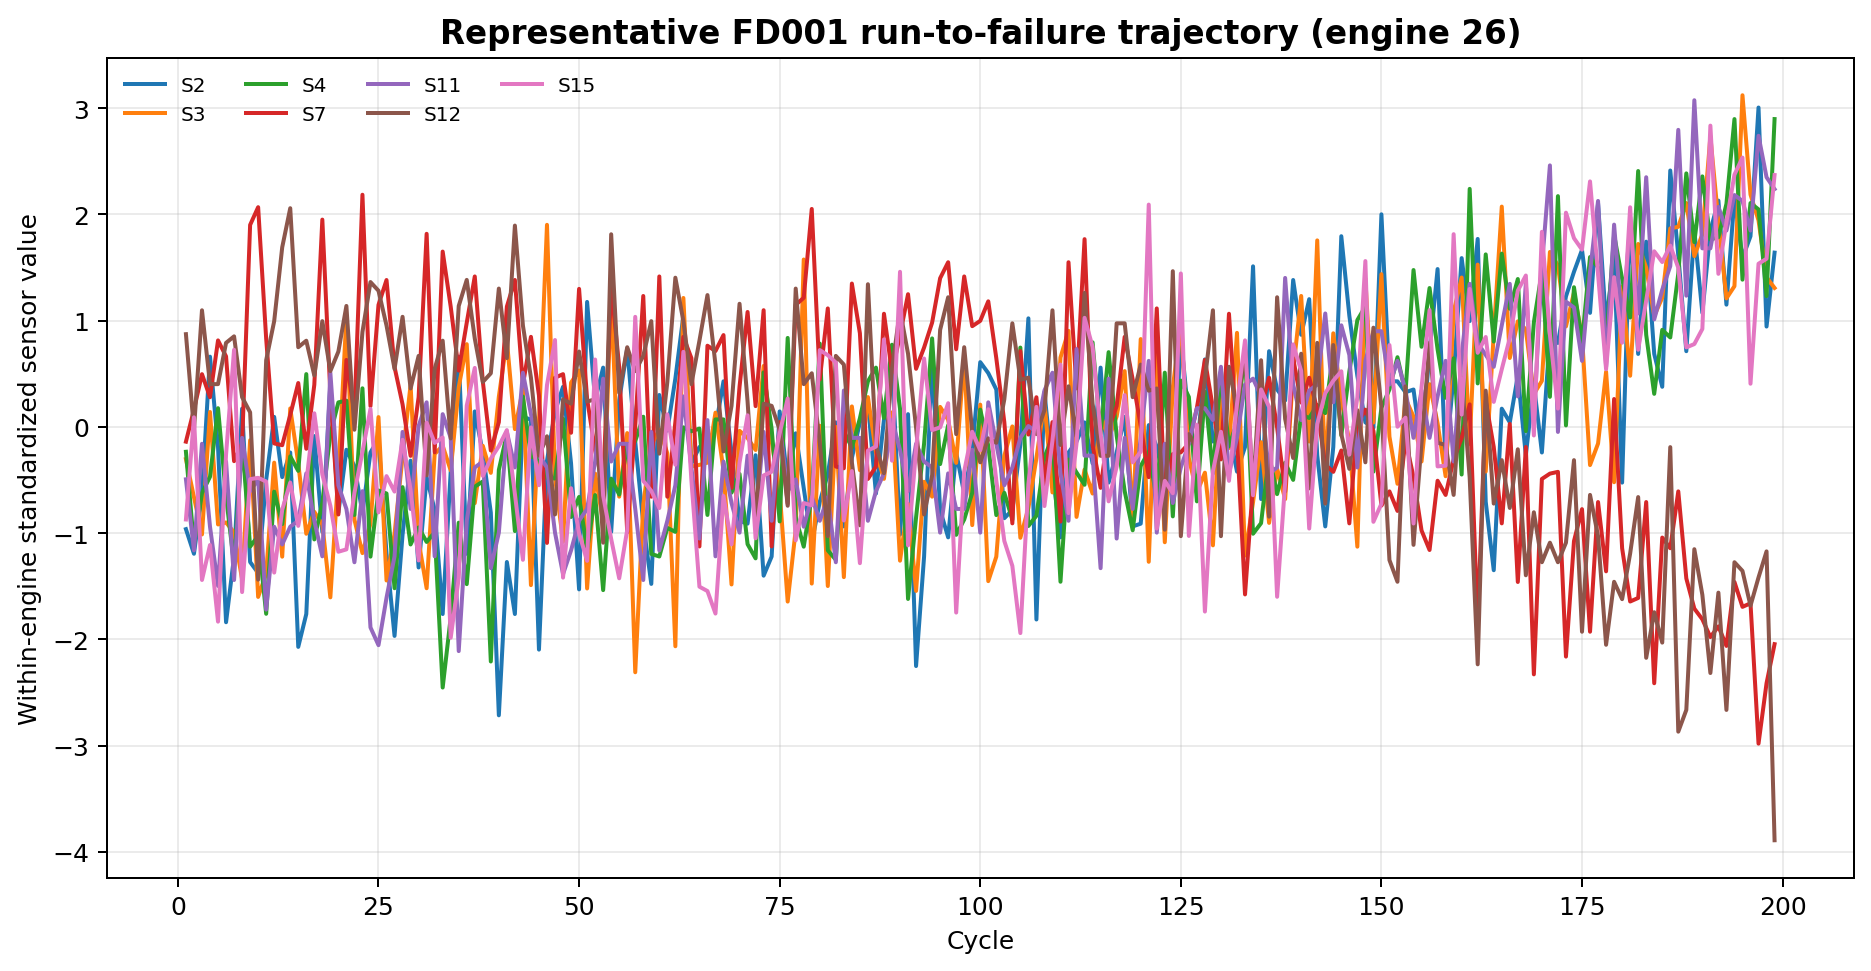
\includegraphics[width=0.92\textwidth]{figures/engine_trajectory.png}
    \caption{Representative engine trajectory from the local CMAPSS data. Sensor values are standardized within the selected engine only for visualization.}
    \label{fig:engine_trajectory}
\end{figure}

\subsection{Derivative Features}
First- and second-order differences are included because RUL is tied not only to the current operating state but also to how that state is changing. A sensor value may remain within a broad operating range while its slope or curvature begins to shift near late degradation. Velocity features expose local rate of change, while acceleration features expose changes in that rate. Figure~\ref{fig:derivative_features} illustrates the relationship between a normalized sensor channel, its first difference, and its second difference for the same representative engine.

\begin{figure}[htbp]
    \centering
    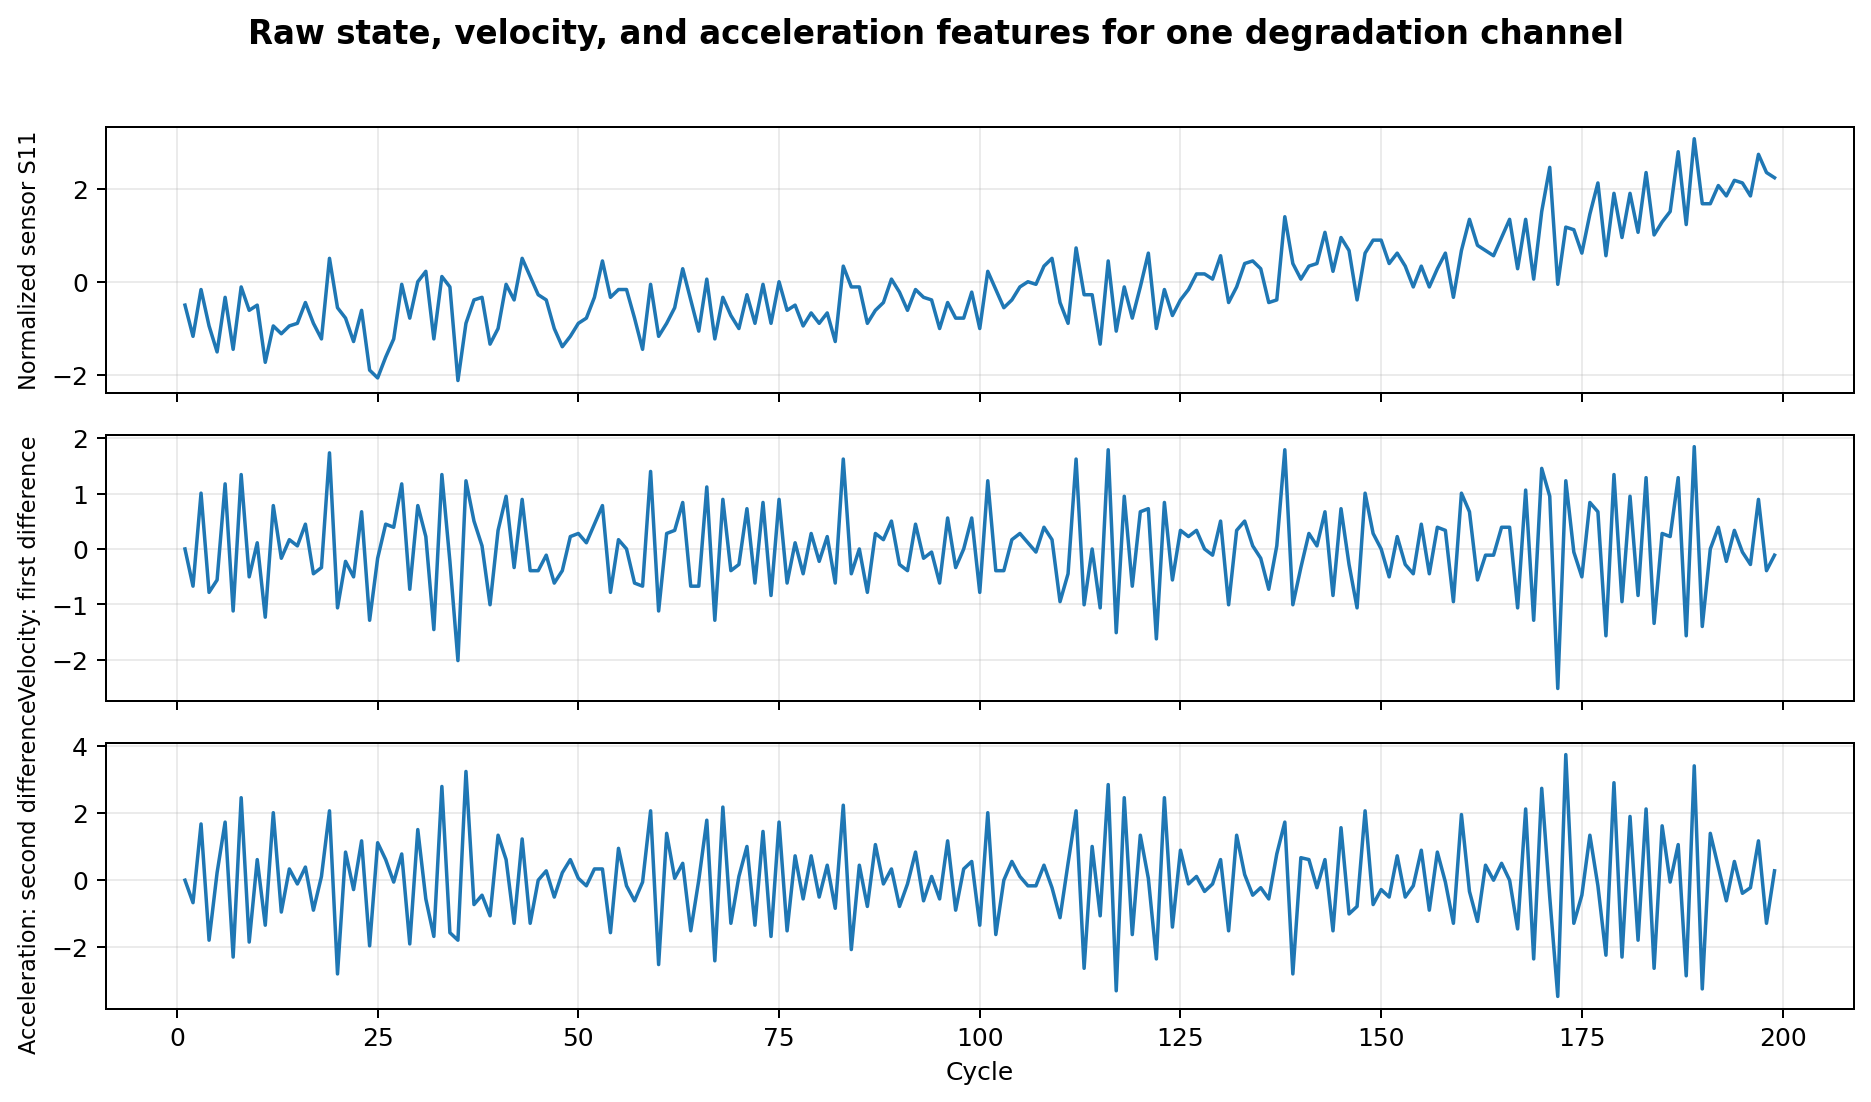
\includegraphics[width=0.9\textwidth]{figures/derivative_features.png}
    \caption{Example of raw state, velocity, and acceleration features used by both model families.}
    \label{fig:derivative_features}
\end{figure}

\subsection{Preprocessing Pipeline}
Figure~\ref{fig:pipeline_diagram} summarizes the shared preprocessing and modeling pipeline. The same normalized and augmented windows are used for both model families, with only the tensor layout and architecture differing between the CNN and Transformer notebooks.

\begin{figure}[htbp]
\centering
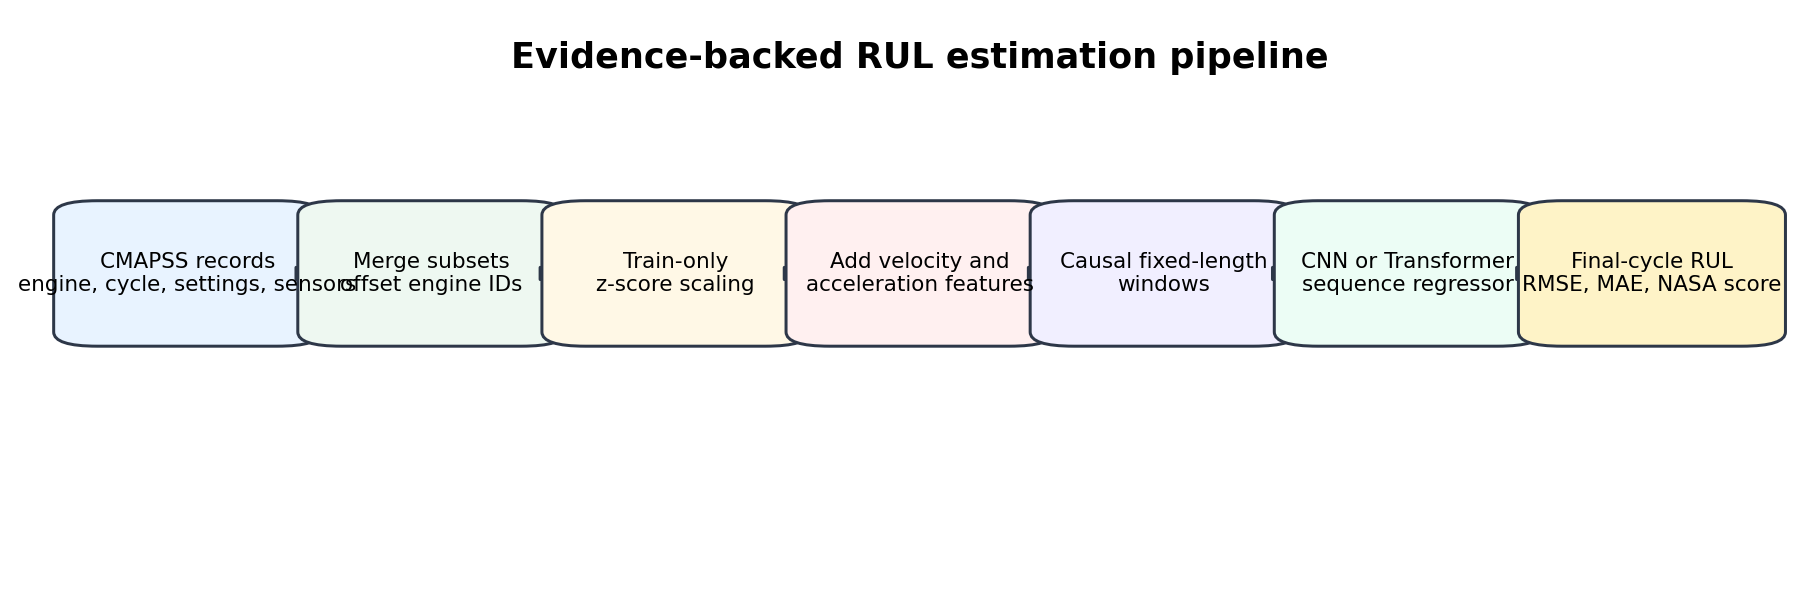
\includegraphics[width=\textwidth]{figures/pipeline_diagram.png}
\caption{Overall RUL estimation pipeline implemented in the notebooks.}
\label{fig:pipeline_diagram}
\end{figure}

\section{Problem Formulation}

Given an observed partial trajectory $(\tilde{x}_{i,1},\dots,\tilde{x}_{i,K_i})$, the goal is to estimate the remaining useful life at the final observed cycle:
\begin{equation}
    f_\theta(\tilde{x}_{i,1},\dots,\tilde{x}_{i,K_i})
    \rightarrow
    \widehat{\mathrm{RUL}}_i.
\end{equation}
The model must satisfy causality: a prediction at cycle $t$ may depend on $\tilde{x}_{i,\tau}$ only for $\tau \leq t$. This constraint is enforced by left-padded causal convolutions in the CNN and by an upper-triangular attention mask in the Transformer.


\newpage


\section{Methodology}

This section describes the shared CMAPSS data pipeline and the two implemented causal sequence models: a dilated causal convolutional neural network and a causal Transformer. The notation, model components, losses, and metrics follow the corresponding notebooks and their recorded experiment outputs.

\subsection{Dataset Representation and Preprocessing}

Each CMAPSS engine is represented as an independent multivariate trajectory. Let $i \in \{1,\dots,N\}$ index engines and let $t \in \{1,\dots,L_i\}$ denote the operating cycle of engine $i$. At each cycle, the observation vector is
\begin{equation}
    x_{i,t} \in \mathbb{R}^{24},
\end{equation}
where the 24 input channels consist of three operational settings and 21 sensor measurements. The full trajectory of engine $i$ is denoted
\begin{equation}
    X_i = (x_{i,1}, x_{i,2}, \dots, x_{i,L_i}).
\end{equation}

Both notebooks standardize features using statistics computed only from the training split. For feature $j$, the normalized value is
\begin{equation}
    \bar{x}_{i,t}^{(j)}
    =
    \frac{x_{i,t}^{(j)} - \mu_j}{\sigma_j},
    \qquad j=1,\dots,24,
\end{equation}
where $\mu_j$ and $\sigma_j$ are the training-set mean and standard deviation of feature $j$. Very small standard deviations are replaced by 1.0 in the implementation to avoid numerical instability.

To expose local degradation dynamics, both models augment the normalized features with first- and second-order temporal differences:
\begin{equation}
    v_{i,t} =
    \begin{cases}
        0, & t=1,\\
        \bar{x}_{i,t} - \bar{x}_{i,t-1}, & t>1,
    \end{cases}
\end{equation}
and
\begin{equation}
    a_{i,t} =
    \begin{cases}
        0, & t=1,\\
        v_{i,t} - v_{i,t-1}, & t>1.
    \end{cases}
\end{equation}
This matches the notebooks' use of \texttt{np.diff(..., prepend=first)}, which makes the first difference vector zero at the start of each engine sequence. The final model input at each cycle is
\begin{equation}
    \tilde{x}_{i,t} =
    [\bar{x}_{i,t}; v_{i,t}; a_{i,t}].
\end{equation}
Since both velocity and acceleration augmentation are enabled in all sampled experiments, this representation supplies the models with the normalized operating state, local rate of change, and local change of rate.

\subsection{RUL Target and Window Construction}

For training trajectories, the RUL target is computed from the final observed training cycle of each engine and capped at $R_{\max}=2000$:
\begin{equation}
    y_{i,t} = \min(L_i - t, R_{\max}).
\end{equation}
For a test engine, the true remaining life after the last observed cycle is supplied by the CMAPSS test labels. If $K_i$ is the last observed cycle and $R_i^{\mathrm{test}}$ is the label for the final observed cycle, the per-cycle target used internally is
\begin{equation}
    y_{i,t}
    =
    \min\left(R_i^{\mathrm{test}} + (K_i - t), R_{\max}\right).
\end{equation}

Training samples are fixed-length windows. For a window length $T$ and stride $s$, a training sample beginning at cycle $r$ is
\begin{equation}
    W_{i,r}
    =
    (\tilde{x}_{i,r}, \tilde{x}_{i,r+1}, \dots, \tilde{x}_{i,r+T-1}),
\end{equation}
with the corresponding RUL sequence
\begin{equation}
    Y_{i,r}
    =
    (y_{i,r}, y_{i,r+1}, \dots, y_{i,r+T-1}).
\end{equation}
Training windows are generated with the sampled stride, while validation and test evaluation use the final available window for each engine. This mirrors deployment: the model observes the latest available operating history and returns the RUL estimate at the last observed cycle.

\subsection{Dilated Causal Convolutional Model}

The convolutional notebook implements a stack of causal one-dimensional convolutions over time. The input tensor is arranged as $(B,C,T)$, where $B$ is batch size, $C$ is the augmented feature dimension, and $T$ is the window length. For layer $\ell \in \{0,\dots,L-1\}$, the dilation is
\begin{equation}
    d_\ell = 2^\ell.
\end{equation}
The convolution uses left-only padding of $(k-1)d_\ell$ samples for kernel size $k$, so the output at time $t$ depends only on current and past values. In mathematical form, the hidden state of a causal convolutional layer can be written as
\begin{equation}
    h_{t}^{(\ell)}
    =
    \phi\left(
        \sum_{m=0}^{k-1}
        W_{\ell,m} h_{t-md_\ell}^{(\ell-1)}
        + b_\ell
    \right),
\end{equation}
where unavailable past values are supplied by left padding and $\phi$ is the GELU nonlinearity used in the notebook. Each convolutional block applies batch normalization before convolution, followed by GELU and dropout.

The effective receptive field of the convolutional stack is
\begin{equation}
    R_{\mathrm{CNN}}
    =
    1 + \sum_{\ell=0}^{L-1}(k-1)2^\ell.
\end{equation}
Predictions before this receptive field is fully populated are partially influenced by padding; therefore, the convolutional loss masks the first $R_{\mathrm{CNN}}-1$ positions in each window. After the convolutional backbone, the hidden representation is transposed to $(B,T,H)$ and passed through a regression head:
\begin{equation}
    \hat{y}_{i,t}^{\mathrm{CNN}}
    =
    g_{\mathrm{CNN}}(h_{i,t}^{(L)}).
\end{equation}
The head consists of layer normalization, a linear projection to half the hidden width, GELU, dropout, and a final linear projection to one scalar RUL value.

\begin{figure}[htbp]
\centering
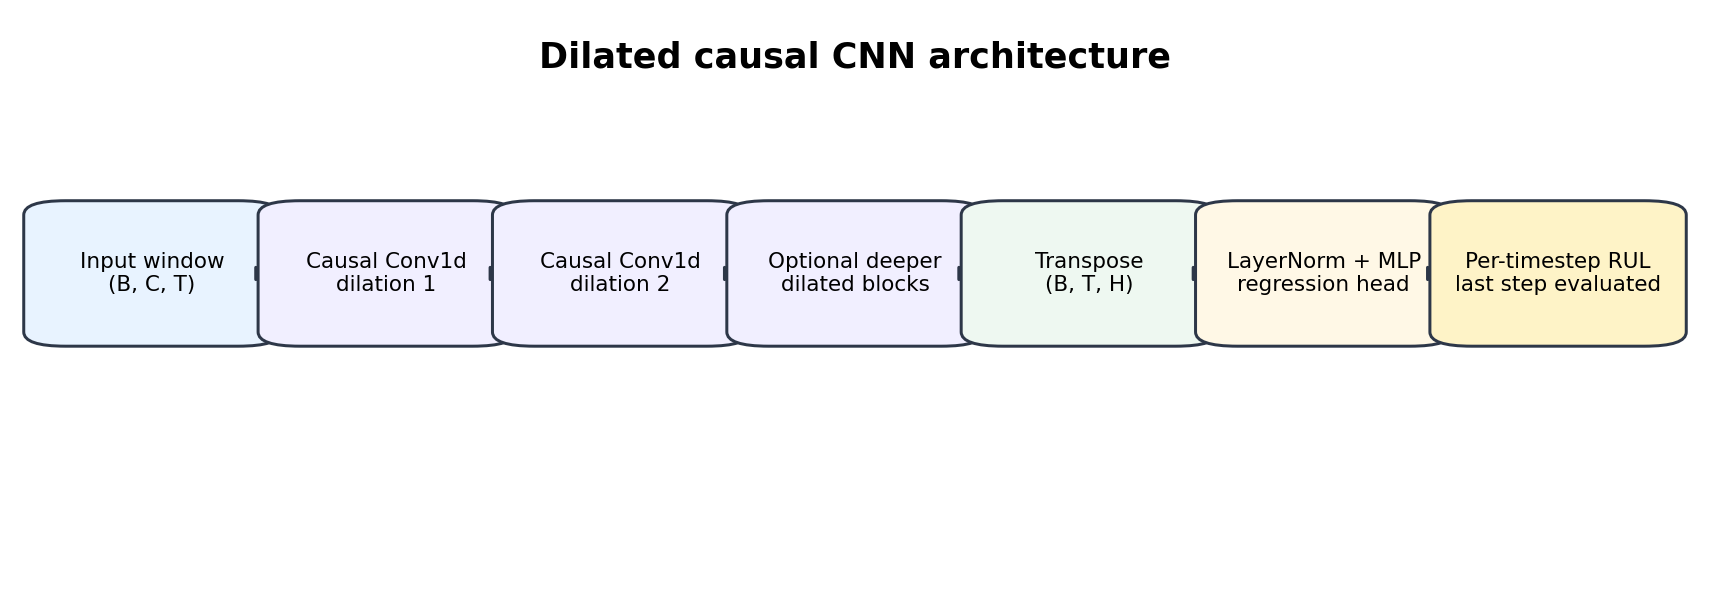
\includegraphics[width=\textwidth]{figures/cnn_architecture.png}
\caption{Causal CNN architecture implemented in the convolution notebook.}
\label{fig:cnn_architecture}
\end{figure}

\subsection{Causal Transformer Model}

The Transformer notebook implements a causal self-attention model over the same augmented sequences, using tensors arranged as $(B,T,C)$. Each input vector is first linearly projected into a latent space:
\begin{equation}
    z_{i,t}^{(0)} = W_e \tilde{x}_{i,t} + b_e.
\end{equation}
Fixed sinusoidal positional encodings are added to preserve temporal order:
\begin{equation}
    h_{i,t}^{(0)} = z_{i,t}^{(0)} + p_t.
\end{equation}

Each Transformer layer applies masked multi-head self-attention followed by a position-wise feed-forward block. For one attention head, queries, keys, and values are
\begin{equation}
    Q = HW_Q,\qquad K = HW_K,\qquad V = HW_V.
\end{equation}
Causal attention is computed as
\begin{equation}
    \operatorname{Attn}(Q,K,V)
    =
    \operatorname{softmax}
    \left(
        \frac{QK^\top}{\sqrt{d_k}} + M
    \right)V,
\end{equation}
with the upper-triangular mask
\begin{equation}
    M_{t,\tau} =
    \begin{cases}
        0, & \tau \leq t,\\
        -\infty, & \tau > t.
    \end{cases}
\end{equation}
This prevents the prediction at cycle $t$ from attending to future cycles in the same window. The implementation uses PyTorch's \texttt{TransformerEncoder} with this causal mask, batch-first tensors, pre-normalized Transformer blocks, GELU activation, dropout, and a feed-forward dimension of $4d_{\mathrm{model}}$.

After $L$ Transformer layers, a regression head maps each hidden state to a scalar prediction:
\begin{equation}
    \hat{y}_{i,t}^{\mathrm{Tr}} = g_{\mathrm{Tr}}(h_{i,t}^{(L)}).
\end{equation}
The head consists of layer normalization, a linear projection to $d_{\mathrm{model}}/2$, GELU, dropout, and a final linear projection. Since every Transformer position can attend to all previous positions immediately through the causal mask, the notebook sets the Transformer receptive-field warmup parameter to $1$.

\begin{figure}[htbp]
\centering
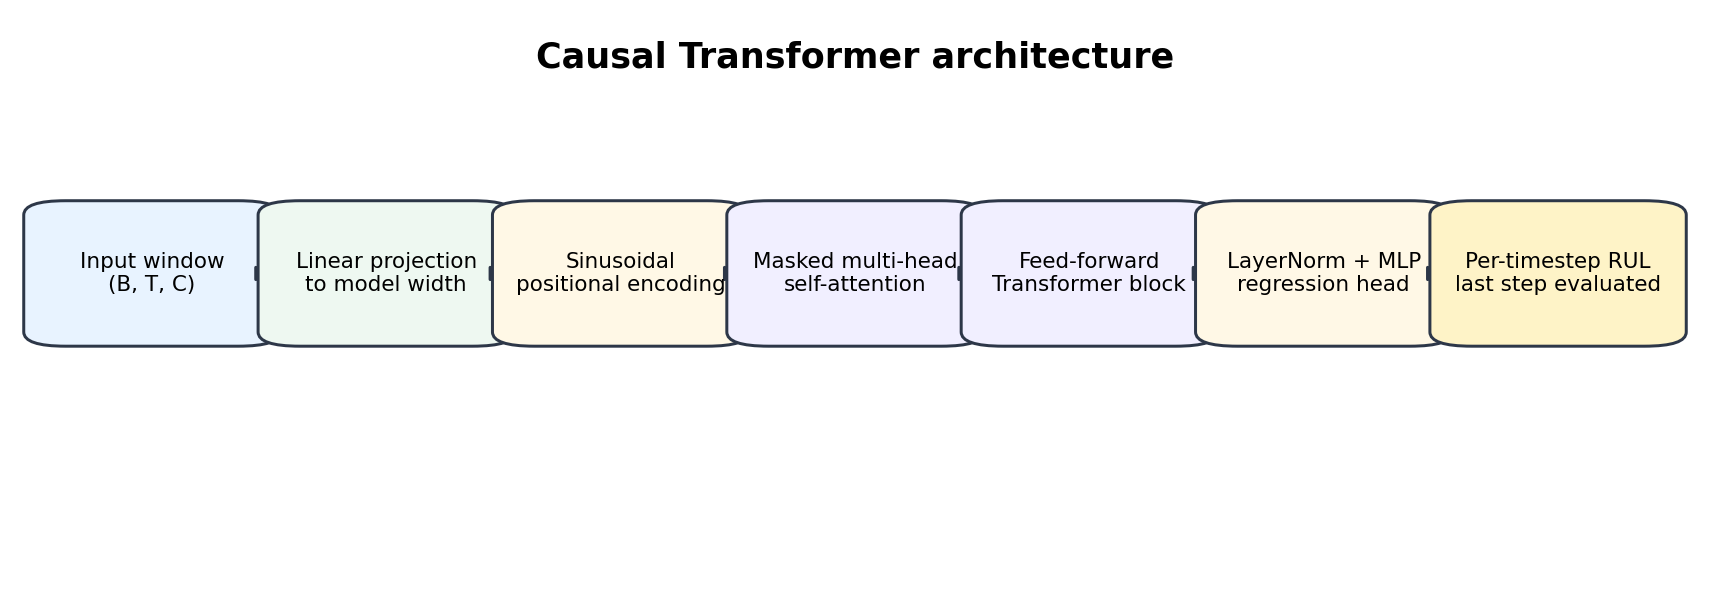
\includegraphics[width=\textwidth]{figures/transformer_architecture.png}
\caption{Causal Transformer architecture implemented in the Transformer notebook.}
\label{fig:transformer_architecture}
\end{figure}

\subsection{Training Objective and Evaluation Metrics}

Both notebooks train with a masked, time-weighted mean squared error. For a batch of padded windows, let $m_{b,t} \in \{0,1\}$ indicate whether timestep $t$ is valid for batch element $b$. Later timesteps are weighted more heavily using
\begin{equation}
    w_t = \exp\left(\beta \frac{t}{T-1}\right),
    \qquad t=0,\dots,T-1.
\end{equation}
Let $r$ denote the model-specific warmup region: $r=R_{\mathrm{CNN}}$ for the convolutional model and $r=1$ for the Transformer. The valid mask used in the loss is
\begin{equation}
    \tilde{m}_{b,t} =
    \begin{cases}
        0, & t < r-1,\\
        m_{b,t}, & t \geq r-1.
    \end{cases}
\end{equation}
The resulting objective is
\begin{equation}
    \mathcal{L}
    =
    \frac{
        \sum_b \sum_{t=0}^{T-1}
        \tilde{m}_{b,t} w_t
        \left(\hat{y}_{b,t} - y_{b,t}\right)^2
    }{
        \sum_b \sum_{t=0}^{T-1}
        \tilde{m}_{b,t} w_t
    }.
\end{equation}
This objective reflects the structure of RUL prediction: early-cycle observations often contain limited degradation evidence, whereas later-cycle observations are more informative for final-cycle prognostics.

At inference time, each model processes the final available window of a test engine and only the last prediction is evaluated:
\begin{equation}
    \widehat{\mathrm{RUL}}_i = \hat{y}_{i,K_i}.
\end{equation}
Performance is measured with RMSE, MAE, and the NASA asymmetric score:
\begin{equation}
    \mathrm{RMSE}
    =
    \sqrt{
        \frac{1}{N_{\mathrm{test}}}
        \sum_{i=1}^{N_{\mathrm{test}}}
        \left(\widehat{\mathrm{RUL}}_i-\mathrm{RUL}_i\right)^2
    },
\end{equation}
\begin{equation}
    \mathrm{MAE}
    =
    \frac{1}{N_{\mathrm{test}}}
    \sum_{i=1}^{N_{\mathrm{test}}}
    \left|
        \widehat{\mathrm{RUL}}_i-\mathrm{RUL}_i
    \right|,
\end{equation}
and, with $d_i=\widehat{\mathrm{RUL}}_i-\mathrm{RUL}_i$,
\begin{equation}
    S_i =
    \begin{cases}
        \exp\left(-\dfrac{d_i}{13}\right)-1, & d_i < 0,\\[6pt]
        \exp\left(\dfrac{d_i}{10}\right)-1, & d_i \geq 0,
    \end{cases}
    \qquad
    S = \sum_{i=1}^{N_{\mathrm{test}}} S_i.
\end{equation}
The NASA score penalizes overestimation of RUL more strongly, reflecting the higher risk of predicting more useful life than remains.

\subsection{Computational Considerations}

The causal CNN has computational cost that grows approximately linearly with sequence length for a fixed kernel size and hidden width. Dilation expands temporal coverage without requiring every timestep to interact with every other timestep, making the convolutional model relatively efficient for long windows. The Transformer has a stronger long-range modeling mechanism because each timestep can attend to all earlier timesteps, but self-attention requires an attention matrix over the window and therefore scales quadratically with window length. This creates a trade-off: the CNN is more computationally economical for long histories, while the Transformer offers a more flexible global dependency mechanism at higher memory cost.

\begin{table}[htbp]
\centering
\caption{Qualitative complexity comparison for a window of length $T$, hidden width $H$, kernel size $k$, and $L$ layers.}
\label{tab:complexity}
\begin{tabular}{lll}
\toprule
\textbf{Model} & \textbf{Dominant temporal cost} & \textbf{Practical implication} \\
\midrule
Causal CNN & $O(LT k H^2)$ & Linear in window length for fixed kernel size \\
Causal Transformer & $O(LT^2H + LTH^2)$ & Quadratic attention memory and compute in $T$ \\
\bottomrule
\end{tabular}
\end{table}

\begin{algorithm}[htbp]
\caption{Training and final-window inference protocol}
\label{alg:training}
\begin{algorithmic}[1]
\State Load all CMAPSS subsets and offset engine identifiers across subsets.
\State Split training engines into train and validation groups at the engine level.
\State Compute feature means and standard deviations from the training group only.
\State Normalize features, add velocity and acceleration channels, and construct causal windows.
\For{each sampled configuration}
    \State Train the causal CNN or Transformer with masked time-weighted MSE.
    \State Evaluate validation engines using their final available windows.
    \State Save the checkpoint with the best validation RMSE.
\EndFor
\State Evaluate the selected checkpoint on each test engine using only its final available window.
\end{algorithmic}
\end{algorithm}

\section{Experimental Setup}

Both pipelines were implemented in PyTorch and executed on the merged CMAPSS subsets discovered in the local \texttt{CMaps/} directory. Engine identifiers were offset across subsets to prevent collisions. The training engines were split into training and validation groups at the engine level using an 80/20 split, so windows from the same engine were not mixed across the two splits. Model selection used the best validation RMSE observed during training.

Each model family ran 50 sampled experiments for 200 epochs with the Adam optimizer. The sampling seed schedule was $42+i$ for experiment index $i$, giving seeds 42 through 91. The implementation uses CUDA when available and otherwise falls back to CPU. Both searches used $R_{\max}=2000$ and enabled velocity and acceleration augmentation. Saved configurations and metrics are stored under \texttt{runs\_cmapss/} for the CNN and the corresponding Transformer run directory for the attention model. Table~\ref{tab:search_space} summarizes the sampled hyperparameter ranges.

\begin{table}[htbp]
\centering
\caption{Hyperparameter search spaces used in the convolutional and Transformer notebooks.}
\label{tab:search_space}
\resizebox{\textwidth}{!}{%
\begin{tabular}{lll}
\toprule
\textbf{Hyperparameter} & \textbf{Causal CNN values} & \textbf{Transformer values} \\
\midrule
Window size & 200, 500, 800, 1000 & 200, 500, 800, 1000 \\
Stride & 1, 2, 5 & 50, 60, 70, 80 \\
Batch size & 32, 64, 128, 256 & 32, 64, 128, 256 \\
Learning rate & $10^{-4}$, $3\times10^{-4}$, $5\times10^{-4}$, $8\times10^{-4}$, $10^{-3}$ & Same \\
Weight decay & 0, $10^{-5}$, $10^{-4}$, $10^{-3}$ & Same \\
Time-weight exponent $\beta$ & 0.25, 0.5, 0.75, 1.0, 1.25, 1.5, 1.75, 2.0 & Same \\
Hidden width & 32, 64, 96, 128 & 32, 64, 96, 128 \\
Layers & 2, 3, 4, 5 & 2, 3, 4, 5 \\
Kernel size & 3, 5, 7 & -- \\
Attention heads & -- & 2, 4, 8 \\
Dropout & 0.2, 0.3, 0.5, 0.7, 0.8 & 0.2, 0.3, 0.5, 0.7, 0.8 \\
\bottomrule
\end{tabular}%
}
\end{table}

\section{Results}

\subsection{Overall Comparison}

Table~\ref{tab:best_model_comparison} compares the best recorded run from each model family, ranked by NASA score. The causal CNN achieves the strongest overall result, with lower RMSE, lower MAE, and a lower NASA score than the best Transformer run. The result is consistent across both symmetric error metrics and the asymmetric NASA score, so the CNN is not merely improving one metric at the expense of another.

\begin{table}[htbp]
\centering
\caption{Best recorded configuration from each model family.}
\label{tab:best_model_comparison}
\begin{tabular}{llrrrr}
\toprule
\textbf{Model} & \textbf{Best experiment} & \textbf{Window} & \textbf{Test RMSE} & \textbf{Test MAE} & \textbf{NASA score} \\
\midrule
Causal CNN & exp\_046 & 1000 & 1.0583 & 0.0741 & 10.6022 \\
Transformer & exp\_016 & 1000 & 1.7273 & 0.1495 & 27.9299 \\
\bottomrule
\end{tabular}
\end{table}

\subsection{Best Runs by Model Family}

Table~\ref{tab:cnn_top_results} reports the five best causal CNN configurations. The best model used a window size of 1000, stride 2, batch size 256, learning rate $5\times10^{-4}$, no weight decay, $\beta=2.0$, hidden width 32, two dilated convolutional layers, kernel size 3, and dropout 0.5. Its validation RMSE was 0.0143 and its test NASA score was 10.6022.

\begin{table}[htbp]
\centering
\caption{Top causal CNN runs ranked by NASA score. Results are taken from the saved CNN run CSV.}
\label{tab:cnn_top_results}
\resizebox{\textwidth}{!}{%
\begin{tabular}{lrrrrrrrrrrrrrr}
\toprule
\textbf{Exp.} & \textbf{Win.} & \textbf{Stride} & \textbf{Batch} & \textbf{LR} & \textbf{WD} & $\boldsymbol{\beta}$ & \textbf{Hidden} & \textbf{Layers} & \textbf{Kernel} & \textbf{Drop.} & \textbf{Val RMSE} & \textbf{Test RMSE} & \textbf{Test MAE} & \textbf{NASA} \\
\midrule
exp\_046 & 1000 & 2 & 256 & 0.0005 & 0.0000 & 2.00 & 32 & 2 & 3 & 0.5 & 0.0143 & 1.0583 & 0.0741 & 10.6022 \\
exp\_016 & 800 & 2 & 256 & 0.0008 & 0.0000 & 0.50 & 32 & 5 & 3 & 0.5 & 0.0527 & 1.7350 & 0.1545 & 27.7651 \\
exp\_007 & 1000 & 2 & 256 & 0.0003 & 0.0001 & 0.75 & 64 & 4 & 5 & 0.8 & 0.0646 & 1.7334 & 0.1664 & 28.2897 \\
exp\_008 & 500 & 1 & 256 & 0.0001 & 0.0000 & 0.50 & 64 & 3 & 7 & 0.7 & 0.0782 & 1.7382 & 0.1776 & 29.0770 \\
exp\_009 & 1000 & 5 & 256 & 0.0010 & 0.0001 & 0.25 & 32 & 4 & 3 & 0.5 & 0.1395 & 1.6962 & 0.2198 & 29.9642 \\
\bottomrule
\end{tabular}%
}
\end{table}

Table~\ref{tab:transformer_top_results} reports the five best Transformer configurations. The best Transformer used a window size of 1000, stride 70, batch size 256, learning rate $8\times10^{-4}$, weight decay $10^{-3}$, $\beta=0.25$, $d_{\mathrm{model}}=32$, two Transformer layers, four attention heads, and dropout 0.5.

\begin{table}[htbp]
\centering
\caption{Top Transformer runs ranked by NASA score. Results are taken from the saved Transformer run CSV.}
\label{tab:transformer_top_results}
\resizebox{\textwidth}{!}{%
\begin{tabular}{lrrrrrrrrrrrrrr}
\toprule
\textbf{Exp.} & \textbf{Win.} & \textbf{Stride} & \textbf{Batch} & \textbf{LR} & \textbf{WD} & $\boldsymbol{\beta}$ & $\boldsymbol{d_{\mathrm{model}}}$ & \textbf{Layers} & \textbf{Heads} & \textbf{Drop.} & \textbf{Val RMSE} & \textbf{Test RMSE} & \textbf{Test MAE} & \textbf{NASA} \\
\midrule
exp\_016 & 1000 & 70 & 256 & 0.0008 & 0.0010 & 0.25 & 32 & 2 & 4 & 0.5 & 0.0136 & 1.7273 & 0.1495 & 27.9299 \\
exp\_039 & 500 & 70 & 256 & 0.0003 & 0.0001 & 2.00 & 32 & 4 & 2 & 0.5 & 0.0244 & 1.7560 & 0.1858 & 30.2536 \\
exp\_010 & 1000 & 60 & 256 & 0.0001 & 0.0001 & 0.75 & 32 & 4 & 8 & 0.8 & 0.2544 & 1.7382 & 0.1975 & 31.5440 \\
exp\_049 & 1000 & 70 & 256 & 0.0003 & 0.0010 & 0.75 & 96 & 5 & 4 & 0.7 & 0.2094 & 1.7568 & 0.2628 & 35.5437 \\
exp\_009 & 1000 & 80 & 256 & 0.0010 & 0.0001 & 0.25 & 32 & 4 & 8 & 0.5 & 0.3406 & 1.7839 & 0.4173 & 42.9590 \\
\bottomrule
\end{tabular}%
}
\end{table}

\subsection{Sensitivity Analysis}

Figure~\ref{fig:result_distributions} summarizes the distribution of test RMSE values across the 50 sampled configurations per model family. The spread is large for both searches, which means the reported best models should be interpreted as selected configurations from a stochastic hyperparameter search rather than as inevitable outcomes of the architecture alone.

\begin{figure}[htbp]
    \centering
    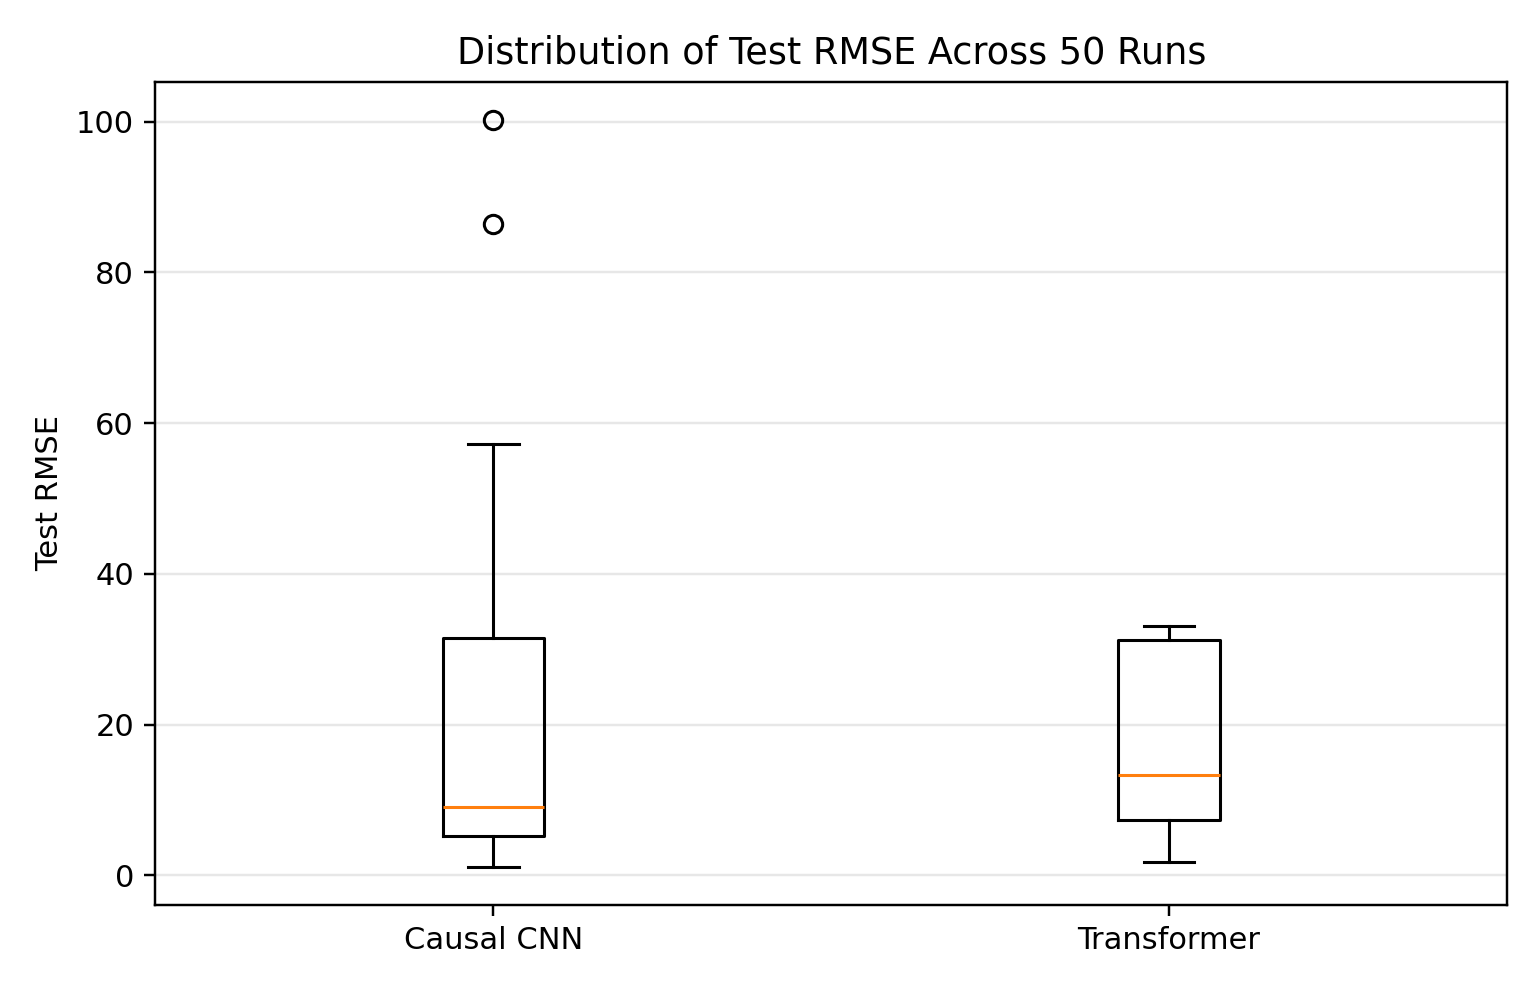
\includegraphics[width=0.82\textwidth]{figures/rmse_distribution.png}
    \caption{Distribution of test RMSE values across the 50 sampled configurations for each model family.}
    \label{fig:result_distributions}
\end{figure}

Window length is the clearest sensitivity pattern in the saved results. For the CNN, the median RMSE improves from 33.5079 at window size 200 to 3.5596 at window size 1000. For the Transformer, the median RMSE improves from 32.7237 at window size 200 to 2.6804 at window size 1000. Figure~\ref{fig:window_sensitivity} shows the same effect visually. Longer windows are useful because late-cycle RUL estimation benefits from a longer observed degradation history, especially when the model uses derivative features.

\begin{figure}[htbp]
    \centering
    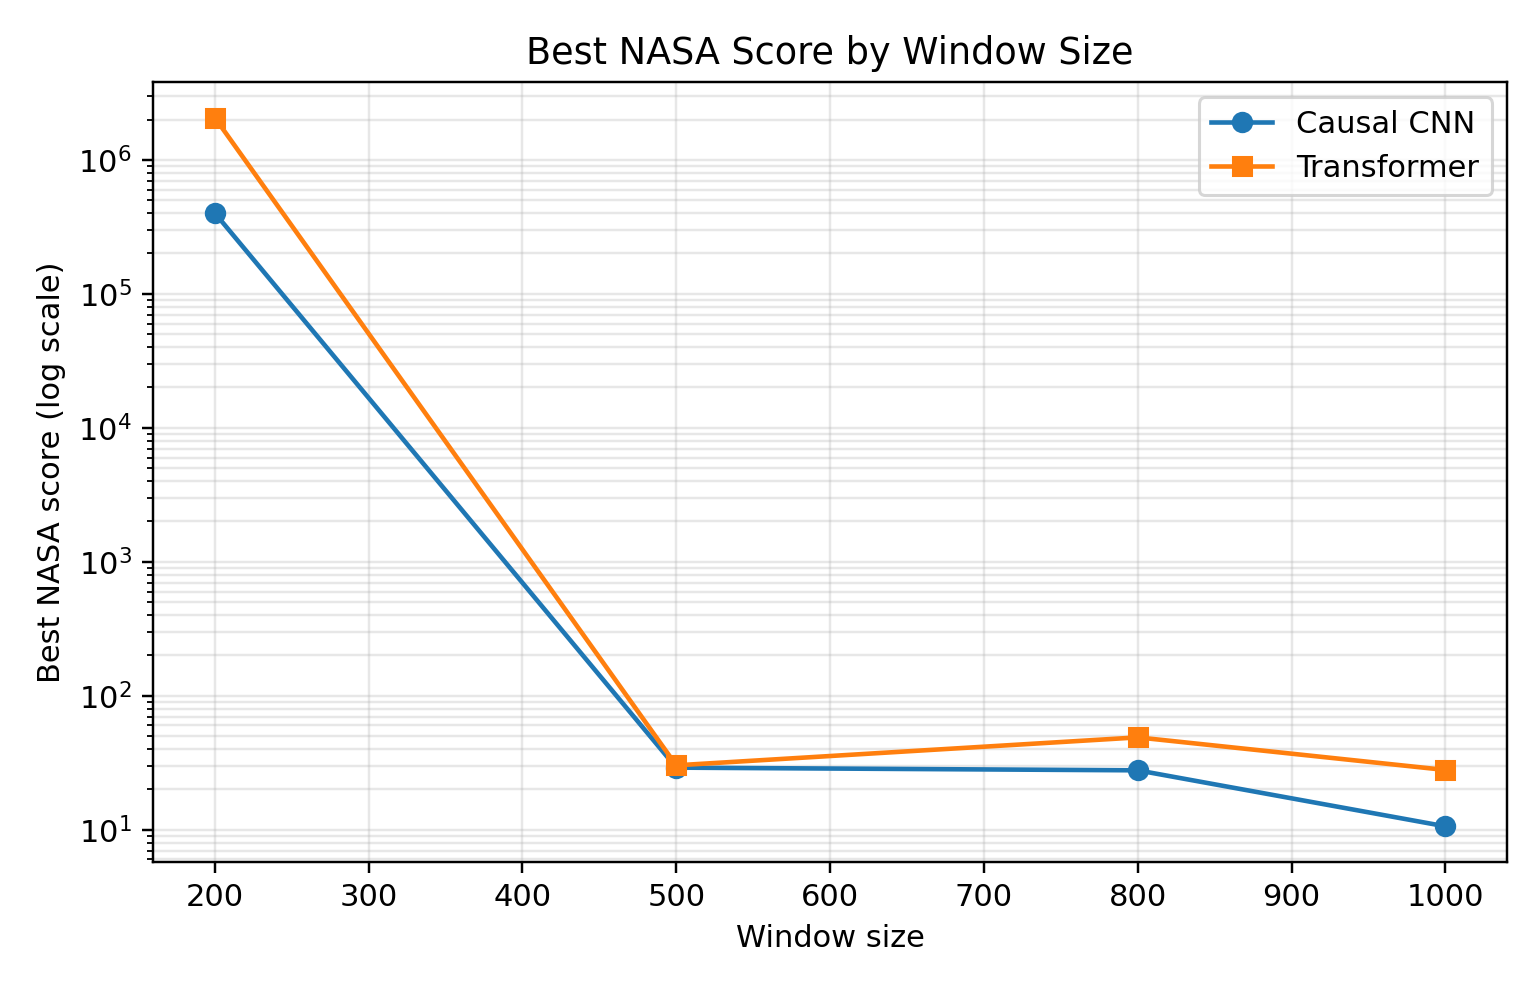
\includegraphics[width=0.82\textwidth]{figures/window_sensitivity.png}
    \caption{Sensitivity of test RMSE to window size across sampled CNN and Transformer configurations.}
    \label{fig:window_sensitivity}
\end{figure}

Dropout also affects stability. For the CNN, dropout 0.5 gives the best median RMSE among the sampled values, with median RMSE 1.7350 and median NASA score 29.9642. For the Transformer, the best single run also uses dropout 0.5, although the median Transformer RMSE at this dropout is 14.3710, indicating that dropout alone does not determine success. Hidden width shows a weaker pattern: the best runs for both model families use width 32, while larger widths do not consistently improve the median result. This suggests that the merged CMAPSS task is not simply capacity-limited under the implemented pipeline.

Figure~\ref{fig:rmse_nasa_scatter} compares RMSE and NASA score. The relationship is positive but not linear because the NASA score is asymmetric and exponential. Configurations with moderate RMSE can still receive very large NASA scores if their errors include risky overestimation of remaining life.

\begin{figure}[htbp]
    \centering
    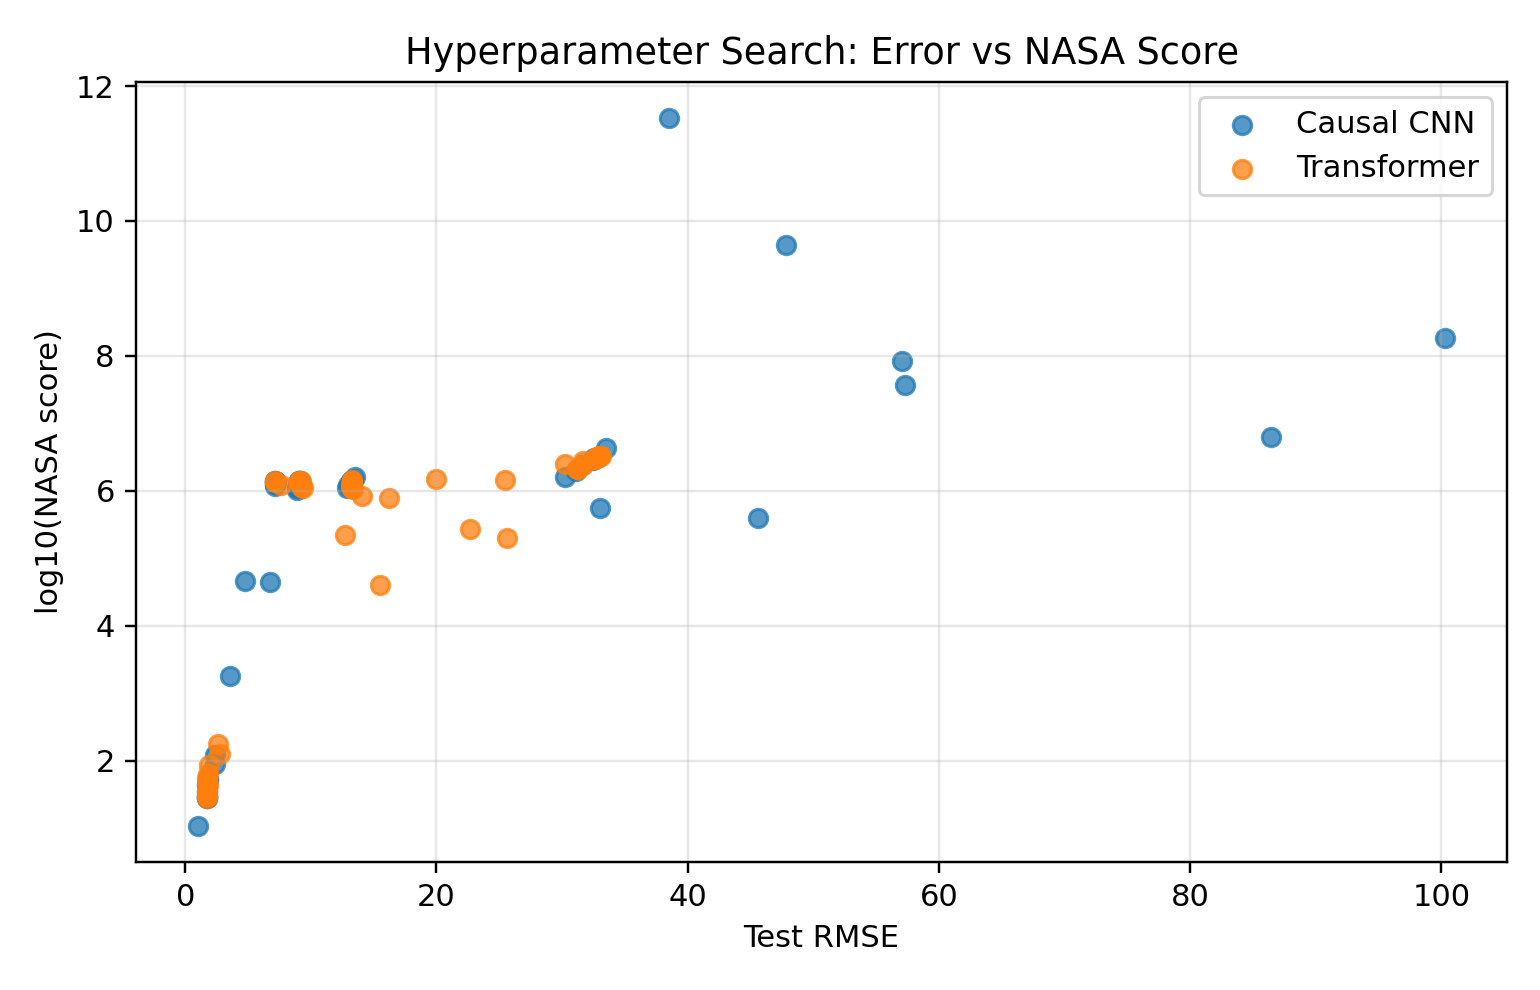
\includegraphics[width=0.82\textwidth]{figures/rmse_nasa_scatter.png}
    \caption{Relationship between RMSE and NASA asymmetric score across sampled configurations.}
    \label{fig:rmse_nasa_scatter}
\end{figure}

\subsection{Error Behavior and Training Curves}

The best CNN has the lowest NASA score, which is important because the NASA metric penalizes RUL overestimation more strongly than underestimation. In maintenance terms, overestimation is more dangerous: a model that predicts too much remaining life can delay maintenance beyond the true failure point. Underestimation is still undesirable because it can cause early maintenance, but it is less severe in the NASA scoring function.

The worst CNN by NASA score is exp\_037, with test RMSE 38.4943, MAE 29.1333, and NASA score approximately $3.41\times10^{11}$. The worst CNN by RMSE is exp\_027, with RMSE 100.2669 and MAE 89.6458. For the Transformer, exp\_048 is worst by both RMSE and NASA score, with RMSE 33.0754, MAE 12.7370, and NASA score approximately $3.29\times10^6$. These failed configurations are concentrated at short windows, especially window size 200, supporting the interpretation that insufficient temporal context can lead to unsafe RUL behavior.

The saved artifacts do not include per-engine prediction files, so this report does not claim engine-level case studies. The error analysis is therefore restricted to aggregate behavior supported by the recorded metrics. Figure~\ref{fig:training_curves} includes the saved training-history plots for the best CNN and Transformer runs, providing a qualitative view of convergence and validation behavior.

\begin{figure}[htbp]
    \centering
    \begin{subfigure}{0.48\textwidth}
        \centering
        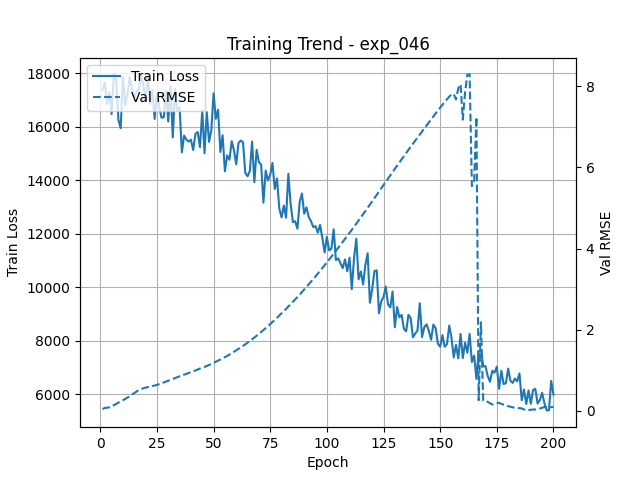
\includegraphics[width=\linewidth]{runs_cmapss/exp_046/history.png}
        \caption{Causal CNN training history.}
    \end{subfigure}
    \hfill
    \begin{subfigure}{0.48\textwidth}
        \centering
        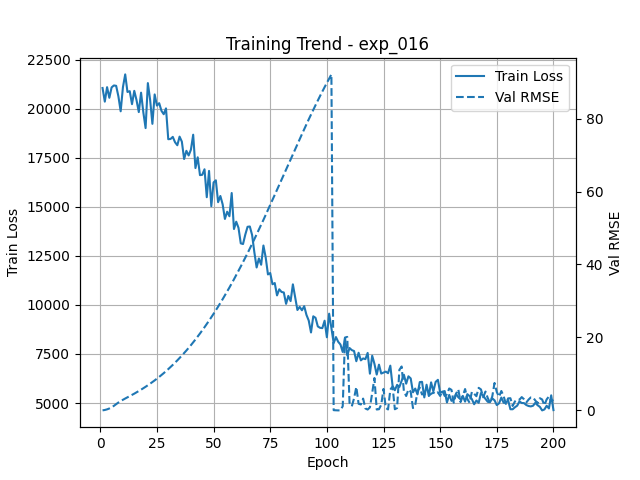
\includegraphics[width=\linewidth]{runs_cmapss_Tranformers/exp_016/history.png}
        \caption{Transformer training history.}
    \end{subfigure}
    \caption{Training loss and validation RMSE history for the best recorded CNN and Transformer configurations.}
    \label{fig:training_curves}
\end{figure}

\section{Sensitivity / Ablation Limitations}

The available saved experiments support sensitivity analysis rather than a complete ablation study. All 100 recorded runs use both velocity and acceleration features, and all sampled configurations use a positive time-weighting exponent $\beta$. Therefore, the report does not claim a raw-only, velocity-only, acceleration-only, or no-time-weight ablation. The defensible conclusion is narrower: within the implemented feature pipeline, performance is highly sensitive to window size, dropout, model width, optimization settings, and model selection.

The strongest evidence from the current artifacts is that longer windows consistently help both architectures, and that the best CNN combines a long window with a compact convolutional backbone. The derivative features remain theoretically motivated and consistently present in the implementation, but their isolated contribution would require additional controlled runs that disable velocity and acceleration channels.

\section{Discussion}

The implemented pipelines treat RUL estimation as causal sequence regression. This is essential for predictive maintenance because a deployable model cannot use future measurements when estimating the current health state. The CNN enforces causality through left-padded dilated convolutions, while the Transformer enforces causality through an upper-triangular attention mask. Both models therefore produce predictions that depend only on current and previous cycles.

The shared time-weighted objective is consistent with degradation physics. Early engine cycles often resemble healthy operation and may carry limited information about exact failure time. Later cycles contain stronger degradation signatures, so increasing the regression weight across the window encourages the models to focus on the portion of the trajectory most relevant to final RUL estimation. The CNN additionally masks early predictions that are still within the convolutional warmup region, avoiding loss contributions from outputs influenced by padding.

The best CNN likely wins because the task rewards local temporal pattern extraction over unrestricted pairwise attention. With velocity and acceleration channels already exposing local degradation dynamics, a compact dilated convolution can combine neighboring trends efficiently and with fewer optimization degrees of freedom. The Transformer has a more flexible dependency mechanism, but the saved search shows that this flexibility does not automatically translate to better final-window RUL estimates under the sampled configurations.

The results also show why the NASA score should be interpreted alongside RMSE and MAE. RMSE measures average squared error, while the NASA score encodes a maintenance preference: overestimating RUL is worse than underestimating it. This is why failed runs can produce extremely large NASA scores even when their RMSE values are not the largest in the entire search. For a prognostics pipeline, this safety-oriented asymmetry is not a detail; it changes which model behavior is acceptable.

\section{Limitations}

The results come from sampled hyperparameter experiments rather than exhaustive searches. Therefore, the reported best models should be interpreted as the best recorded configurations from the implemented notebooks, not as globally optimal architectures. The unusually large NASA scores in some failed runs also indicate that the asymmetric metric can become very large when a model substantially overestimates RUL.

The experimental artifacts do not include controlled raw-only, derivative-only, or no-time-weight runs, so this report cannot isolate the independent causal contribution of each preprocessing component. The saved artifacts also do not include per-engine prediction files, which prevents a fully grounded case-study analysis of the hardest engines without rerunning inference from checkpoints.

Finally, all experiments are conducted on CMAPSS simulation data. Real flight data would introduce maintenance interventions, sensor replacement, calibration drift, missing values, and distribution shifts across aircraft and operating regimes. A deployable system would need validation under these conditions and would likely require uncertainty estimates or conservative decision thresholds in addition to point RUL predictions.

\section{Conclusion}

This work implements and compares two causal deep learning frameworks for RUL estimation on CMAPSS turbofan degradation trajectories. Both models combine train-only standardization, dynamics-based feature augmentation, causal temporal modeling, time-weighted regression, and final-window inference. The best causal CNN achieves the strongest recorded result, with test RMSE 1.0583, MAE 0.0741, and NASA score 10.6022. The best Transformer also performs strongly, achieving test RMSE 1.7273, MAE 0.1495, and NASA score 27.9299.

The main empirical pattern is that long causal windows and compact temporal models are effective for this pipeline. Future work should add controlled ablations for raw features, velocity, acceleration, and time weighting; save per-engine predictions for case-study analysis; repeat the best configurations across multiple seeds; and add sensor-level interpretability analyses to identify which measurements drive late-stage RUL predictions.

\begin{thebibliography}{9}

\bibitem[Saxena et~al.(2008)]{saxena2008damage}
Saxena, A., Goebel, K., Simon, D., and Eklund, N. (2008).
\newblock Damage propagation modeling for aircraft engine run-to-failure simulation.
\newblock In \emph{2008 International Conference on Prognostics and Health Management}, pages 1--9. IEEE.

\bibitem[Vaswani et~al.(2017)]{vaswani2017attention}
Vaswani, A., Shazeer, N., Parmar, N., Uszkoreit, J., Jones, L., Gomez, A. N., Kaiser, L., and Polosukhin, I. (2017).
\newblock Attention is all you need.
\newblock In \emph{Advances in Neural Information Processing Systems}, volume 30.

\bibitem[Zheng et~al.(2017)]{zheng2017long}
Zheng, S., Ristovski, K., Farahat, A., and Gupta, C. (2017).
\newblock Long short-term memory network for remaining useful life estimation.
\newblock In \emph{2017 IEEE International Conference on Prognostics and Health Management}, pages 88--95.

\bibitem[Malhotra et~al.(2016)]{malhotra2016lstm}
Malhotra, P., Ramakrishnan, A., Anand, G., Vig, L., Agarwal, P., and Shroff, G. (2016).
\newblock LSTM-based encoder-decoder for multi-sensor anomaly detection.
\newblock In \emph{ICML 2016 Anomaly Detection Workshop}.

\bibitem[Bai et~al.(2018)]{bai2018empirical}
Bai, S., Kolter, J. Z., and Koltun, V. (2018).
\newblock An empirical evaluation of generic convolutional and recurrent networks for sequence modeling.
\newblock \emph{arXiv preprint arXiv:1803.01271}.

\end{thebibliography}

\end{document}
